\renewcommand{\theequation}{\theenumi}
\renewcommand{\thefigure}{\theenumi}
\renewcommand{\thetable}{\theenumi}
\begin{enumerate}[label=\thesection.\arabic*.,ref=\thesection.\theenumi]
\numberwithin{equation}{enumi}
\numberwithin{figure}{enumi}
\numberwithin{table}{enumi}

\item The probability that a part manufactured by a company will be defective is 0.05. If 15 such parts are selected randomly and inspected,the probability that atleast two parts will be defective is \dots
%
\\
\solution
%
The desired probabilty is 
\begin{align}
    \pr{X \ge 2 } &= 1 - \pr{X < 2 }
    \\
    &= 1-\pr{X=0}-\pr{X=1}
    \\
    &= 1-\comb{15}{0} p^{0} q^{15} -\comb{15}{1} p^{1} q^{14}
    \\
    &=0.1709   
\end{align}
%
where 
\begin{align}
    p = 0.0.5, q = 1-p = 0.95
\end{align}
%
and $X$ is binomial with parameters $\brak{15, p}$.

%
\item Let $X$ be a binomial random variable with parameters \brak{11,\frac{1}{3}}. At which value(s) of $k$ is \pr{X=k} maximized?\\
\begin{enumerate}
\item $k=2$ 
\item $k=3$ 
\item $k=4$ 
\item $k=5$
\end{enumerate}
%
\solution
%

The binomial distribution is given by:
\begin{equation}
\pr{X=k}=\comb{n}{k}\times p^k\times q^{n-k}
\end{equation}
We are given $n=11$, $p=\frac{1}{3}$ and hence $q=\frac{2}{3}$
\begin{align}
\pr{X = k}={\comb{11}{k}}\brak{\frac{2}{3}}^{11-k}\brak{\frac{1}{3}}^{k}
\end{align}
%To maximise $\pr{X = k}$,
\begin{align}
%\pr{X = k}&\geq\pr{X = k+1}\\
\frac{\pr{X = k}}{\pr{X = k+1}} &\geq1
\\
\implies \frac{{\comb{11}{k}}\brak{\frac{2}{3}}^{11-k}\brak{\frac{1}{3}}^{k}}{{\comb{11}{k+1}}\brak{\frac{2}{3}}^{10-k}\brak{\frac{1}{3}}^{k+1}}&\geq1
\\
\text{or, }k&\geq3
\label{binom/2/condition1}
\end{align}
after some algebra.  Similarly, 
\begin{align}
%\frac{2(k+1)}{11-k}&\geq1\\
%\pr{X = k}&\geq\pr{X = k-1}\\
\frac{\pr{X = k}}{\pr{X = k-1}}& \geq 1\\
% \implies \frac{12-k}{2k}&\geq1\\
% &=\frac{{\comb{11}{k}}\brak{\frac{2}{3}}^{11-k}\brak{\frac{1}{3}}^{k}}{{\comb{11}{k-1}}\brak{\frac{2}{3}}^{12-k}\brak{\frac{1}{3}}^{k-1}}
k&\leq4\label{binom/2/condition2}
\end{align}
From \eqref{binom/2/condition1} and \eqref{binom/2/condition2},  it is obvious that $\pr{X = k}$ is maximized for $k=3$, $k=4$. Hence, options 2 and 3 are correct.  See Fig. 
\ref{binom/2/fig:binom dist} for a graphical verification.
%\renewcommand{\thefigure}{1}
\begin{figure}[!htb]
\centering
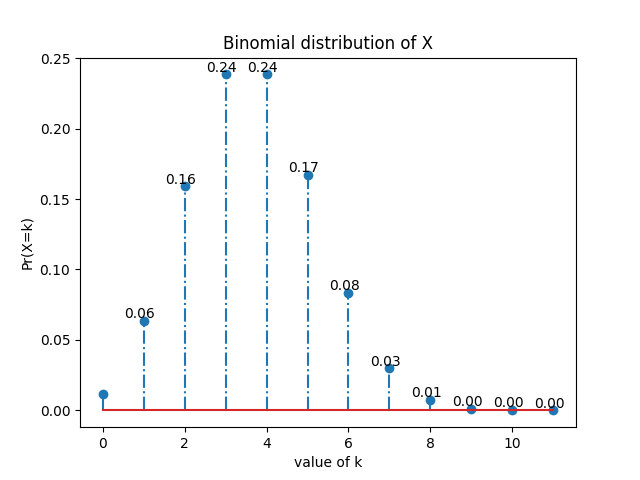
\includegraphics[width=\columnwidth]{binomial/solutions/2/Binomial-stemplot.png}
\caption{Binomial Distribution of  $X$}
\label{binom/2/fig:binom dist}
\end{figure}


%
\item The probability that a ticketless traveler is caught during a trip is 0.1. If the traveler makes 4 trips , the probability that he/she will be caught during at least one of the trips is:\\
\begin{enumerate}
    \item $1-(0.9)^4$
    \item $(1-0.9)^4$
    \item $1-(1-0.9)^4$
    \item $(0.9)^4$
\end{enumerate}
\solution
Let $X_i\in\cbrak{0,1}$ represent the ith trip where 1 denotes a ticketless traveller is caught.
Given,
\begin{align}
     \pr{X_i=1}&=p=0.1 \label{dec2015-3:a}
\end{align}
Let,
\begin{align}
    X=\sum_{i=1}^n X_i
\end{align}
where n is the number of trips and X has a binomial distribution.
\begin{align}
    p_X(k)&=
    \begin{cases}
     \comb{n}{k}\,p^K(1-p)^{n-k}, & 0\le k\le n
     \\
    0, & otherwise
    \end{cases}\label{dec2015-3:z}
\end{align}
As he/she makes 4 trips in total, Using \eqref{dec2015-3:a} and
\eqref{dec2015-3:z},
\begin{align}
    \pr{X=0}&=p_X(0)\\
    &=\comb{4}{0}\,p^0(1-p)^4\\
    \pr{X=0}&=(0.9)^4\label{dec2015-3:2}
\end{align}
Then probability of being caught in atleast one trip is,(Using \eqref{dec2015-3:2})
\begin{align}
    \pr{X\ge1}&=1-\pr{X<1}\\
    &=1-\pr{X=0}\label{dec2015-3:1}\\
    &=1-(0.9)^4
\end{align}
%
\item Let X be a binomial random variable with parameters  $\brak{11,\displaystyle{\frac{1}{3}}}$. At which value(s) of k is $\Pr\brak{X = k}$ maximized?\\
\begin{enumerate}
\item k=2
\item k=3
\item k=4
\item k=5
\end{enumerate}
%
\solution
X has a binomial distribution :
\begin{align}
\Pr\brak{X=k} = {\comb{n}{k}}(q)^{n-k}(p)^{k}
\end{align}
Where,
\begin{itemize}
\item n=11
\item $\displaystyle{p=\frac{1}{3}}$
\item $\displaystyle{q=1-p=1-\frac{1}{3}=\frac{2}{3}}$
\end{itemize}
\begin{align}
\Pr\brak{X = k}={\comb{11}{k}}\left(\frac{2}{3}\right)^{11-k}\left(\frac{1}{3}\right)^{k}
\end{align}
For Pr(X = k) to be maximized
\begin{align}
\Pr\brak{X = k}\:\geq\:\Pr\brak{X = k+1}\\
\frac{\Pr\brak{X = k}}{\Pr\brak{X = k+1}}=\frac{{\comb{11}{k}}\left(\frac{2}{3}\right)^{11-k}\left(\frac{1}{3}\right)^{k}}{{\comb{11}{k+1}}\left(\frac{2}{3}\right)^{10-k}\left(\frac{1}{3}\right)^{k+1}}\geq1
\end{align}
\begin{align}
\frac{2(k+1)}{11-k}\geq1\\
\implies k\geq3\label{dec2012-104:0.0.7}\\
\Pr\brak{X = k}\:\geq\:\Pr\brak{X = k-1}\\
\frac{\Pr\brak{X = k}}{\Pr\brak{X = k-1}}=\frac{{\comb{11}{k}}\left(\frac{2}{3}\right)^{11-k}\left(\frac{1}{3}\right)^{k}}{{\comb{11}{k-1}}\left(\frac{2}{3}\right)^{12-k}\left(\frac{1}{3}\right)^{k-1}}\geq1\\
\frac{12-k}{2k}\geq1\\
\implies k\leq4\label{dec2012-104:0.0.10}
\end{align}
From \eqref{dec2012-104:0.0.7} , \eqref{dec2012-104:0.0.10} and since k is an integer\\
$\Pr\brak{X = k}$ is maximized for k=3, k=4\\
Thus options 2) and 3) are correct\\


\end{enumerate}